\section{Описание алгоритма}
    Дана матрица $A$ и столбец $b$ и система $Ax = b$. Суть метода выбора главного элемента в том, что на каждом шаге находится максимальный элемент матрицы, после чего из всех строк вычитается главная строка, умноженная на коэффициент для того чтобы получить нули в главном столбце. 
    
    Далее, на $k$-том шаге в необработанных до этого строках системы находится максимальный по модулю элемент. Пусть это будет элемент $a_{ij}$. Из каждой другой необработанной $l$-той строки вычитается данная строка, умноженная на $\frac{a_{lj}}{a_{ij}}$, тем самым получая нули в $j$-том столбце данных строк.

    В итоге, после $n-1$ шага получается матрица, которую можно решить путём исключения переменных.

\pagebreak

\section{Тестирование}
    Для тестирования будут сгенерированы случайные матрицы и столбцы размерностью 10 в количестве 10000. (код алгоритма см. в приложении)

    \begin{figure}[H]
        \centering
        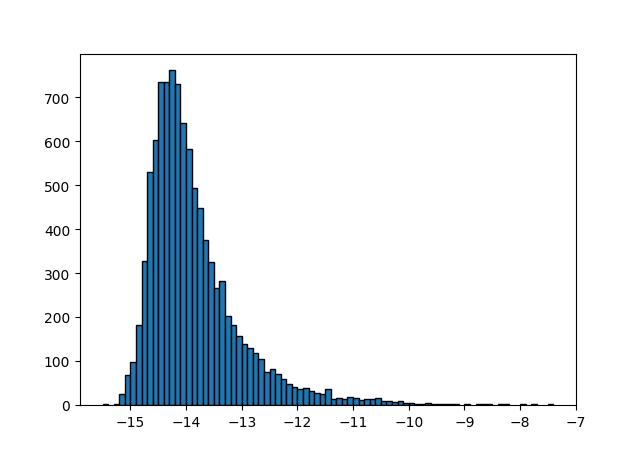
\includegraphics[width=16cm]{pictures/BarCounts.png}
        \caption{Log10 максимальной разницы решения алгоритма и встроенной функции numpy, округлённый до десятых при генерации 10000 случайных матриц.}
    \end{figure}

    На рисунке 1 можно увидеть распределения точностей решения. Большинство решений по точности не превышает $10^{-10}$. Решения с меньшей точностью определяются большим числом обусловленности сгенерированной матрицы -- от 2000 до 31000. Однако, количество таких решений -- $29$, что составляет всего $0.29 \% $ от всех решений.

    \begin{figure}[H]
        \centering
        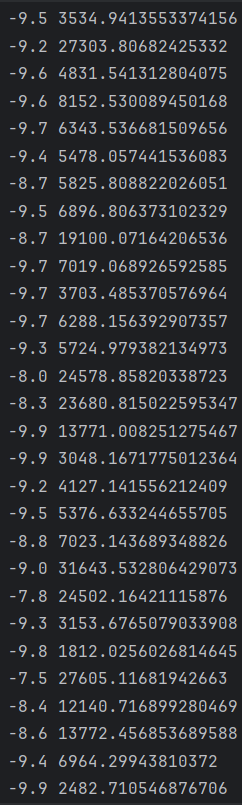
\includegraphics[width=6cm]{pictures/BigConditions.png}
        \caption{Log10 разности и число обусловленности решений, которые не превысили точность $10^{-10}$.}
    \end{figure}